\scanpage{14}
c)
\[
\begin{aligned}
\unsure{\mathfrak{S}|\mathcal{S}}_4&\simeq\operatorname{Aff}\,2,\mathbb{F}_2)\simeq\operatorname{GP}(1,\mathbb{F}_3)\\
\unsure{\mathfrak{A}|\mathcal{A}}_4&\simeq\operatorname{Aff}(1,\mathbb{F}_4)\qquad ?
\end{aligned}
\]

% Two detached points at the right of c), between its two formula baselines;
% writing versus surface trace remains uncertain, with no punctuation assigned.
\margin{\figure{\unsure{\begin{tikzpicture}[x=1mm,y=1mm]
\fill (0,1.2) ellipse [x radius=.15,y radius=.19];
\fill[gray] (-.04,0) ellipse [x radius=.13,y radius=.22];
\end{tikzpicture}}}}

d)
\[
\begin{aligned}
\mathfrak{S}_5&\simeq\operatorname{GP}(1,\mathbb{F}_5)\\
\mathfrak{A}_5&\simeq\operatorname{GP}(1,\mathbb{F}_4)
\end{aligned}
\]

Some classical groups over a field $k$

\diagram{\(\left.
\begin{tikzcd}[ampersand replacement=\&,column sep=small,row sep=1em]
1\arrow[r] \& k^*\arrow[r] \& \operatorname{Gl}(V)\arrow[r] \&\operatorname{GP}(V)\arrow[r,dash]\&1\\
1\arrow[r] \& k^*\arrow[r,dash] \&\operatorname{Gl}(n,k)\arrow[r] \&\operatorname{GP}(n-1,k)\arrow[r]\&1
\end{tikzcd}
\right\}\;\text{does not \unsure{split} in general}\)}

% slanted, in the left margin; the surrounding line has small gaps at the left.
\reversemarginpar
\margin{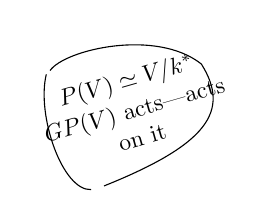
\begin{tikzpicture}[baseline=(proj.base),rotate=16,scale=.85]
\node[inner sep=2pt,transform shape] (proj) {\shortstack{$\mathbb{P}(V)\simeq V/k^*$\\$\operatorname{GP}(V)$ \unsure{acts|acts}\\on it}};
\draw (-1.05,.88) .. controls (-.75,1.12) and (.65,1.05) .. (1.15,.35)
  .. controls (1.38,-.45) and (.9,-.83) .. (-.75,-1.0);
\draw (-1.12,.84) .. controls (-1.43,.3) and (-1.37,-.9) .. (-.95,-1.0);
\end{tikzpicture}}
\normalmarginpar

\[
\begin{aligned}
\text{Structure of a $k$-vector space }\tikz[baseline=(vectbase.base)]{
  \node[inner sep=0pt] (vectbase) {on set};
  \node[anchor=south west,inner sep=0pt] at ([xshift=-.3em,yshift=.8em]vectbase.north west) {\inserted{of dimension $n$}};
  \draw ([xshift=-.35em,yshift=-.4em]vectbase.west)
    .. controls ([xshift=-.7em,yshift=1.0em]vectbase.west) and ([xshift=.4em,yshift=1.1em]vectbase.north west)
    .. ([xshift=.35em,yshift=1.1em]vectbase.north east)
    .. controls ([xshift=.6em,yshift=1.15em]vectbase.north east) and ([xshift=.6em,yshift=1.35em]vectbase.north east)
    .. ([xshift=.4em,yshift=1.35em]vectbase.north east);
}V
&\longleftrightarrow\ \text{datum of \unsure{an|an} \unsure{element|element|element|element}}\\
&\qquad\text{of }\operatorname{Isom}_{\text{ens}}(k^n,V)/\operatorname{Gl}(n,k)
\end{aligned}
\]

Structure of a $k$-affine space of dimension $n$ on \deleted{$E$} set $E$
\[
\begin{aligned}
\longleftrightarrow\ &\text{datum of an \unsure{element|element} of}\\
&\operatorname{Isom}_{\text{ens}}(k^n,V)/\unsure{\operatorname{Aff}n,k)|\operatorname{Aff}(n,k)}
\end{aligned}
\]

[ In \unsure{general|general}, \deleted{if $Z$ is a \unsure{group|group}}, the notion of
\tikz[baseline=(oldaff.base)]{
  \node[inner sep=0pt] (oldaff) {\deleted{\unsure{affine|affine} space}};
  \node[anchor=south west,inner sep=0pt] at ([xshift=.8em,yshift=.7em]oldaff.north west)
    {\inserted{torsor (on the right, say) $E$}};
}
under an unspecified \unsure{group|group} can be considered as structure on the underlying set $E$ alone,
\tikz[baseline=(oldapp.base)]{
  \node[inner sep=0pt] (oldapp) {\deleted{\unsure{namely map} $E\times E\times E\,\unsure{\mathbin{\text{---}}|\longrightarrow}\,E$}};
  \node[anchor=south west,inner sep=0pt] at ([xshift=.7em,yshift=.7em]oldapp.north west)
    {\inserted{for example datum of a}};
}
\deleted{$(x,y,z)\,\unsure{\mathrel{\mapstochar\relbar\joinrel\relbar}|\longmapsto}\,\unsure{6x|sx|\delta x}$}
pair $\Gamma\subset\mathfrak{S}_{E}$ subgroup, such that \ldots ] ; \unsure{valid} for sets with a \uline{faithful} group of operators\ldots ]

A structure of an \uline{affine space under} $k$ is then the datum of such a $\Gamma$, with \deleted{\unsure{$\Gamma$ commutative}} commutative, \unsure{\deleted{and}|and} a homomorphism of unital rings.
\[
 k\longrightarrow\operatorname{End}_{\mathbb{Z}}(\Gamma)\quad\ldots\qquad ]
\]

Structure of a $k$-projective space of dimension $n$ on $\unsure{P|\mathbb P}$
\[
\begin{tikzpicture}[baseline=(projective.base)]
\node[anchor=base west,inner sep=0pt] (projective) at (0,0)
 {$\displaystyle\longleftrightarrow\quad\text{datum of}\quad
 \operatorname{Isom}_{\text{\unsure{ens|ens,}}}\left(
 \underset{\substack{\rotatebox{90}{$=$}\\(k^n-\unsure{(0)|(0}/k^*}}{\mathbb{P}^{n-1}(k)},P\right)
 /\operatorname{GP}(n-1,k)$};
% The enclosure over the arrow is open at its top, not a closed box.
\node[inner sep=0pt,font=\small] at (.35,.70) {definition};
\draw (.02,.87) -- (.02,.45) -- (.68,.45) .. controls (.75,.45) and (.75,.64) .. (.75,.86);
\draw[->] (.36,.45) -- (.36,.12);
% Divider bends below the small quotient and continues rightward.
\draw (2.70,-.77) -- (6.00,-.77)
 .. controls (6.35,-.77) and (6.25,-1.17) .. (6.70,-1.17) -- (11.60,-1.17);
\end{tikzpicture}
\]

\diagram{\begin{tikzcd}[ampersand replacement=\&,column sep=small,row sep=.6em]
\operatorname{Gl}(n,k)\arrow[r]\&\operatorname{Aff}(n,k)\arrow[r]\&\operatorname{GP}(n,k)\\
\substack{\text{vector space of dimension $n$}\\\text{over $k$}}\arrow[r,maps to,"\substack{\text{forgetting}\\\text{origin}}"']
\&\substack{\text{affine space of}\\\text{dimension $n$ over $k$}}
\arrow[r,maps to,"\substack{\text{projective space}\\\text{associated with}\\\text{the \unsure{enveloping|enveloping} vector space}}"']
\&\substack{\text{projective space}\\\text{of dimension $n$ over $k$}}
\end{tikzcd}}
% archive sheet number: 13
